% Chapter 4

\chapter{Implementation}
\label{Chapter4}
\lhead{Chapter 4. \emph{Implementation}}

\section{An example process}
\label{sec:example_process}
To reiterate the more detailed description of trace acquisition, an
example process that we would like to automate consists of the
following steps, assuming that we already have a customized image set
up for our tests, as well as we already have an executable benchmark
application we'd like to run:
\begin{itemize}
\item allocate the specified number of nodes on a specified site
\item deploy our custom image on the allocated nodes
\item create a nodefile containing the names of the allocated nodes
\item broadcast the runnable across the nodes
\item disable all cores but one on every allocated node (see 3.4.1 for
  explanation)
\item run the mpi experiment from a chosen "head" node (can be any of
  the allocated nodes)
\item gather the traces from the allocated nodes to the head node
\item merge the traces
\item convert merged trace file to Paje format
\end{itemize}
As a side note: in this example, we assume that we are working on the
Grid'5000 testbed. As previously mentioned, most of the work regarding
this thesis was conducted there.\\
As for the example process: parameters that the user can give to it
are the number of nodes, the chosen Grid'5000 site, the image to
deploy, the runnable and parameters to mpirun (for example to disable
Infiniband) and the trace\_gather script. The nodefile created in the
3rd step is necessary for the operations that are needed to do
something on all the allocated nodes.\\
Now let's take a look at the experimentation engine we'd like to use
for implementing the framework to automate processes like this.
\section{XPflow}
In 2.8.2, we already discussed business workflows, foreshadowing the
fact that XPflow, the tool used to implement our framework, is based
on that approach, which includes Business Process Modeling and
Management. There are 2 main concepts in XPflow\cite{bn12_2}:
\begin{itemize}
\item Process: It is the high-level description of the experiment,
  written in a DSL, which is embedded in Ruby. Processes are
  responsible for orchestrating activities and other processes,
  creating a workflow.
\item Activities: The low-level building blocks of the
  experiments. They are written in Ruby and used for implementing the
  lower-level details of the experiment, to do the "real work" in it
  (for example: manage files, start the MPI job).
\end{itemize}
Lets take a look at how these concepts are used through
examples, while uncovering a few other possibilities of XPflow.
\subsection{A general example}
First, we examine an example of transforming general, everyday
activities transformed into XPflow (\ref{fig:xpflow_example1}).
\begin{figure}[htbp]
  \centering
    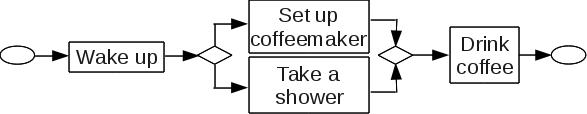
\includegraphics[scale=0.7]{./Figures/xpflow_example1.jpg}
  \caption[dayum]{Morning routine in XPflow}
  \label{fig:xpflow_example1}
\end{figure}
On the diagram, circles represent the starting and end point of the
process, the rectangles represent activities and the whole diagram
represents a process.\\
In XPflow, it is possible to execute activities sequentially or in
parallel. An example for sequential execution on
\ref{fig:xpflow_example1} is drinking coffee: the activities preceding
it must all be finished before that activity can be
started. On the contrary, setting up the coffeemaker and taking a
shower can be executed in parallel, since it's not necessary to stand
by the coffeemaker while it finishes - we can take a shower while it's
running.
\subsection{An MPI experiment example}
After the generic introduction, let's take a look at how we could
represent the experiment we described in section
\ref{sec:example_process} in XPflow. The representation can be seen on
\ref{fig:xpflow_example2}.
\begin{figure}[htbp]
  \centering
    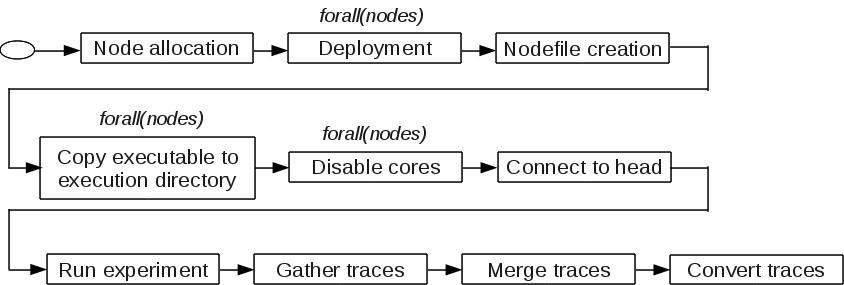
\includegraphics[scale=0.7]{./Figures/xpflow_example2.jpg}
  \caption[dayum]{An MPI experiment in XPflow}
  \label{fig:xpflow_example2}
\end{figure}
On this representation, there is no parallel execution like in the
previous example: one activity has to be executed sequentially after
the other, the activities depend on each other. However, as we can
see, some of the activities are distinguished by the text
"forall(nodes)" above them. This means that we iterate through all the
allocated nodes, executing the activity on all of them. This is done
in parallel.\\
As a side note: in the current implementation, this kind of iteration
is realized not
specifically by XPflow, but by the parallel launching tool mentioned
in \ref{sec:experiment_scheduling}, Taktuk\cite{chr09}. This is simply
because it was simpler to implement it that way, because this is a
known and stable solution, while XPflow is under heavy development
currently, thus its internals are subject to change. However, it could
be done with XPflow-specific funcionalities as well. In the long term,
using XPflow-specific funcionality would make the framework more
generic (less Grid'5000-specific).
